

\documentclass{beamer}

\mode<presentation> {

% The Beamer class comes with a number of default slide themes
% which change the colors and layouts of slides. Below this is a list
% of all the themes, uncomment each in turn to see what they look like.

%\usetheme{default}
%\usetheme{AnnArbor}
%\usetheme{Antibes}
%\usetheme{Bergen}
%\usetheme{Berkeley}
%\usetheme{Berlin}
%\usetheme{Boadilla}
%\usetheme{CambridgeUS}
%\usetheme{Copenhagen}
%\usetheme{Darmstadt}
%\usetheme{Dresden}
%\usetheme{Frankfurt}
%\usetheme{Goettingen}
%\usetheme{Hannover}
%\usetheme{Ilmenau}
%\usetheme{JuanLesPins}
%\usetheme{Luebeck}
%\usetheme{Madrid}
%\usetheme{Malmoe}
%\usetheme{Marburg}
%\usetheme{Montpellier}
%\usetheme{PaloAlto}
%\usetheme{Pittsburgh}
%\usetheme{Rochester}
%\usetheme{Singapore}
%\usetheme{Szeged}
%\usetheme{Warsaw}

% As well as themes, the Beamer class has a number of color themes
% for any slide theme. Uncomment each of these in turn to see how it
% changes the colors of your current slide theme.

%\usecolortheme{albatross}
%\usecolortheme{beaver}
%\usecolortheme{beetle}
%\usecolortheme{crane}
%\usecolortheme{dolphin}
%\usecolortheme{dove}
%\usecolortheme{fly}
%\usecolortheme{lily}
%\usecolortheme{orchid}
%\usecolortheme{rose}
%\usecolortheme{seagull}
%\usecolortheme{seahorse}
%\usecolortheme{whale}
\usecolortheme{wolverine}

%\setbeamertemplate{footline} % To remove the footer line in all slides uncomment this line
%\setbeamertemplate{footline}[page number] % To replace the footer line in all slides with a simple slide count uncomment this line

%\setbeamertemplate{navigation symbols}{} % To remove the navigation symbols from the bottom of all slides uncomment this line
}

\usepackage{graphicx} % Allows including images
\usepackage{booktabs} % Allows the use of \toprule, \midrule and \bottomrule in tables


\usepackage{listings}
\lstset{language=Java,
                basicstyle=\footnotesize\ttfamily,
                keywordstyle=\footnotesize\color{blue}\ttfamily,
}

%----------------------------------------------------------------------------------------
%	TITLE PAGE
%----------------------------------------------------------------------------------------

\title[Packages]{8.Packages} % The short title appears at the bottom of every slide, the full title is only on the title page

\author{Sakib Abrar} % Your name
\institute[BUET] % Your institution as it will appear on the bottom of every slide, may be shorthand to save space
{
CSE\\~\\Bangladesh University of Engineering \& Technology \\ % Your institution for the title page
\medskip
\textit{sakib.cghs@gmail.com} % Your email address
}
\date{\today} % Date, can be changed to a custom date

\begin{document}

\begin{frame}
\titlepage % Print the title page as the first slide
\end{frame}

\begin{frame}
\frametitle{Overview} % Table of contents slide, comment this block out to remove it
\tableofcontents % Throughout your presentation, if you choose to use \section{} and \subsection{} commands, these will automatically be printed on this slide as an overview of your presentation
\end{frame}

%----------------------------------------------------------------------------------------
%	PRESENTATION SLIDES
%----------------------------------------------------------------------------------------

%------------------------------------------------
\section{Package basics}
%------------------------------------------------


\begin{frame}{Package basics}
\begin{itemize}
\item Java package provides a mechanism for par55oning
the class name space into more manageable chunks\\
– Both \textbf{naming} and \textbf{visibility} control mechanism
\item Define classes inside a package that are not
accessible by code outside that package.\\
\item Define class members that are exposed only to other
members of the same package\\
\item This allows classes to have in5mate knowledge of
each other\\
– Not expose that knowledge to the rest of the world.\\
\end{itemize}
\end{frame}


%------------------------------------------------
\section{Declaring Package}
%------------------------------------------------


\begin{frame}{Declaring Package}
\begin{itemize}
\item \textbf{package pkg}\\
– Here, pkg is the name of the package\\
\item \textbf{package MyPackage}\\
– creates a package called MyPackage
\item The package statement defines a name space in
which classes are stored.
\item If you omit the package statement, the class names
are put into the \textbf{default package}, which has no name.
\end{itemize}
\end{frame}


\begin{frame}{Declaring Package}
\begin{itemize}
\item Java uses file system directories to store packages\\
– the .class files for any classes that are part of MyPackage
must be stored in a directory called MyPackage
\item More than one file can include the same package
statement
\item The package statement simply specifies to which
package the classes defined in a file belong
\item To create hierarchy of packages, separate each
package name from the one above it by use of a (.)
\end{itemize}
\end{frame}

%------------------------------------------------
\section{Package Examples}
%------------------------------------------------

\begin{frame}
\frametitle{Package Examples}

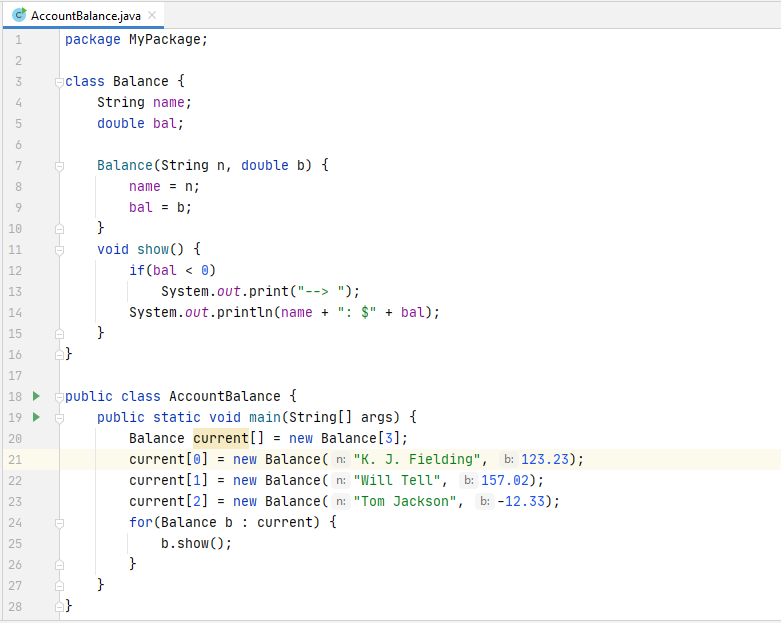
\includegraphics[width=0.95\textwidth]{MyPackage.png}
\end{frame}

%------------------------------------------------

%------------------------------------------------
\section{Access Protection}
%------------------------------------------------

\begin{frame}{Access Protection}
\begin{itemize}
\item Packages act as containers for classes and other
subordinate packages

\item Classes act as containers for data and code
\item The class is Java’s smallest unit of abstraction
\item Four categories of visibility for class members\\
– Subclasses in the same package\\
– Non-subclasses in the same package\\
– Subclasses in different package\\
– Classes that are neither in the same package
subclasses\\
\end{itemize}
\end{frame}

%-------------------------------------------------

%------------------------------------------------

\begin{frame}{Access Protection}
\begin{itemize}
\item The three access modifiers provide a variety of ways
to produce the many levels of access required \\~\\
\textbf{The following applies only to members of classes:}\\~\\
\centerline{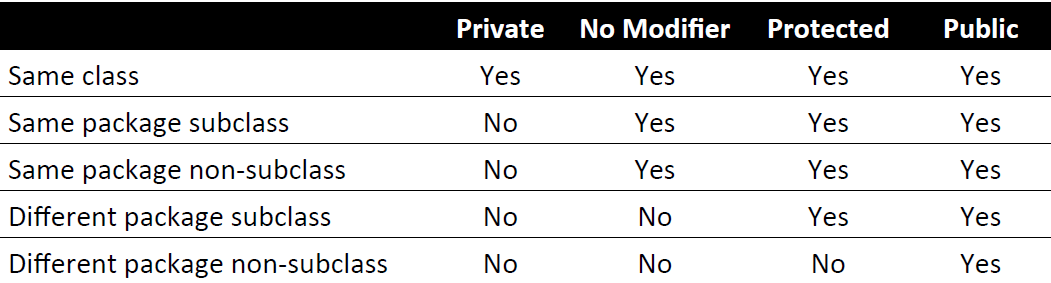
\includegraphics[width=\textwidth]{AccessProtection.png}}
\end{itemize}
\end{frame}

%-------------------------------------------------

%------------------------------------------------

\begin{frame}{Access Protection}
\begin{itemize}
\item Anything declared \textbf{public} can be accessed from
anywhere

\item Anything declared \textbf{private} cannot be seen outside of
its class
\item When a member does not have an explicit access
specifica5on, it is visible to subclasses as well as to
other classes in the same package (\textbf{default access})
\item If you want to allow an element to be seen outside
your current package, but only to classes that subclass
the class directly, then declare that element \textbf{protected}
\end{itemize}
\end{frame}

%-------------------------------------------------

%------------------------------------------------

\begin{frame}{Access Protection}
\begin{itemize}
\item A non-nested class has only two possible access
levels\\
– default and public

\item When a class is declared as public, it is accessible by
any other code
\item If a class has default access, then it can only be
accessed by other code within its same package
\item When a class is public, it must be the only public
class declared in the file, and the file must have the
same name as the class
\end{itemize}
\end{frame}

%-------------------------------------------------

%--------------------------------------------------

\begin{frame}
\Huge{\centerline{THE END }}
\end{frame}

%----------------------------------------------------------------------------------------

\end{document} 